\documentclass[10pt,a4paper]{article}
\usepackage[UTF8]{ctex}
\usepackage{bm}
\usepackage{amsmath}
\usepackage{amsthm}
\usepackage{amssymb}
\usepackage{graphicx}
\title{General Physics: Principle of Homemade Radio}
\author{陈稼霖 \and 45875852}
\date{2018.6.6}
\theoremstyle{remark}
\newtheorem{defi}{Definition}
\newtheorem{cdefi}{\bf 定义}
\begin{document}
\maketitle
无线电广播的目的就是将低频原始信号(电台节目)搭载在高频信号上后在空气中远距离传输至终端(收音机)再解码回低频原始信号,其主要步骤分为调制和解调两个部分。
\section{调制}
无线电台将低频信号转化为高频信号的过程称为调制。
\subsection{利用麦克风将声音信号转化为电信号}
为便于处理与远距离传输,必须首先使用麦克风将声信号(电台节目)转化为电信号。麦克风的原理是法拉第电磁感应原理,如图(\ref{principleOfMicrophone})为麦克风的原理图
\begin{figure}
  \centering
  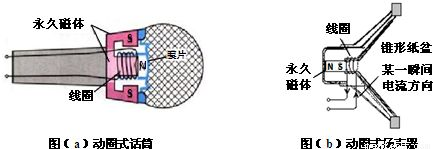
\includegraphics{principleOfMicrophone.jpg}\\
  \caption{收音机原理图}\label{principleOfMicrophone}
\end{figure}
,麦克风的模型图主要由一个永久磁体和一个套在永久磁体上的线圈组成。声音的本质即为空气的振动,具有能量,空气的振动带动线圈同步振动,从而使线圈切割磁感线产生与节目声音相同频率的感应电流。这一步应用到了麦克斯韦方程组中的法拉第电磁感应定律。
\subsection{通过调制将低频信号搭载在高频信号上并利用天线发射}
要将信号发射出去,必须利用天线将电信号其转化为空气中的电磁波。天线可以视为一个带有开放性极板的电容(发射信号的电路中还有一条地线直接连通大地,大地可以看成这个电容的另一个极板),这样开放性的电路可以增大向外发射信号的功率和发射信号的角度范围,通过天线产生的电场的变化产生交替变化的电磁场从而产生电磁波。然而直接发射低频信号是不可行的,而必须转化为高频信号发射,理由有三:1. 为使发射效率足够高,天线长度应当接近信号波长,如最常用的天线--- 半波振子的长度大约为信号波长的四分之一,人能发出声音的频率范围为100Hz 到10000Hz,能听到的声音的频率范围为20Hz 到20000Hz,也就是说天线差不多要4 千米,这显然是不可行的,而高频信号,如我国调幅无线电的频率为$535-1605kHz$,所需天线长度约为$75$ 米,比较符合无线电广播发射塔的尺度,更为可行;2. 难以产生大功率的低频信号,天线产生的电磁波靠的是变化的电流,信号频率小,即天线中电流变化速度较慢,产生的磁场较小,变化的磁场进一步产生的电场也小,故要发射大功率的低频信号所需要很大的电流幅值,在技术上存在较大的难度;3. 频分复用,提高信道容量,不同电台的节目声音在相同的频率范围内,若用低频信号直接发射,则不同电台节目的信号将混在一起,采用高频信号的形式发射,可以使不同节目的信号用不同的频率同时进行发射,防止这些信号串在一起。

因此必须降低频信号搭载在高频信号,这里仅讨论调幅,调幅的过程可以概括为原始信号与一个直流信号相加,再与一个交流信号相乘,考虑一个频率为$f_c$,幅度为$A$的载波(正弦波):
\[
c(t) = A\cdot\sin(2\pi f_ct)
\]
设原始信号的频率为$f_m(\ll f_c)$,幅值为$M(<1)$(保证幅值始终为正,否则在检波时会丢失信息)
\[
m(t) = M\cdot\cos(2\pi f_m + \phi)
\]
将原始信号先加上一个直流信号$(1V)$再与载波信号相乘,得到调制后的高频信号
\[
\begin{split}
y(t) &= [1+m(t)]\cdot c(t)\\
&= [1+M\cdot\cos(2\pi f_mt+\phi)]\cdot\sin(2\pi f_ct)\\
&= A\cdot\sin(2\pi f_ct) + \frac{AM}{2}[sin(2\pi(f_c+f_m)t+\phi) + sin(2\pi(f_c-f_m)t-\phi)]
\end{split}
\]

如图(\ref{highFrequencySignal}) 为搭载了低频信息的高频信号
\begin{figure}
  \centering
  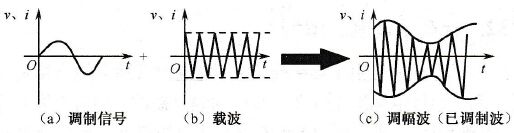
\includegraphics[scale = 1]{highFrequencySignal}\\
  \caption{高频信号(调幅)示意图}\label{highFrequencySignal}
\end{figure}
,其中可以看到调制后的高频信号,一方面以很高的频率上下振动,另一方面其幅度在以较小的频率改变,其改变的幅度(也就是包络面)包含原始信息。
%调制的基本电路比较复杂(图略),大致思想就是利用三极管

\section{解调}
接受高频信号并将其解码为原来的信号的过程称为解调。
\subsection{调谐}
如图(\ref{circuitOfHomemadeRadio})为本无源收音机的电路图,其由自制天线L($20-30\mu H$),可变电容C(大约为$100pF$的微调电容),检波二极管$1N60$,滤波电容$C_1$($2200pF$)无线电发射塔发射的信号在空气中以交替变化的电磁场传播,其通过线圈的磁通量也以图(\ref{highFrequencySignal}) 中高频信号的形式变化,从而根据法拉第电磁感应定律,就可以感应出相同波形的电流。
\begin{figure}
  \centering
  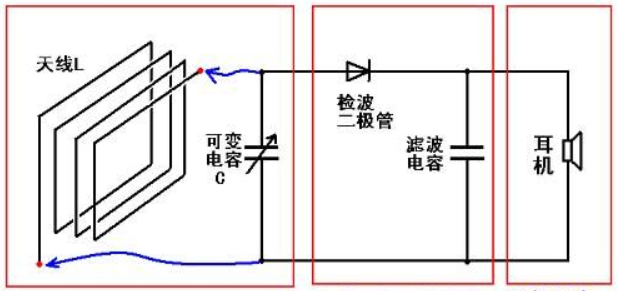
\includegraphics[scale = 0.6]{circuitOfHomemadeRadio}\\
  \caption{收音机电路}\label{circuitOfHomemadeRadio}
\end{figure}

感应产生的电动势随着时间变化而正负交替,而二极管具有单向导电性,当二极管被导通时,可以视为无电阻的导线,整个电路可以视为一个$LRC$振荡电路,其中天线既是产生感应电动势的电源,也是电感,可变电容和定值电容并联形成一个大电容,变压器由于电感较大,而电路中电流电压变化很快,所以通过电流很少,可以粗略视为断路,对左边电路没有影响;当二极管未导通时,电阻极大,可以视为断路,故左边的电路中的一系列电压、电流值等的变化对于右边没有影响,右边电容器缓慢放电。然而空气中存在着各种频道(不同频率)的高频信号,他们都可以在电路中感应出各自频率的感应电流,但是设$LRC$振荡电路的电动势为$V = V_0\cos(\omega t)$,则电路中的电流大小为
\[
I(t) = \frac{V_0}{\sqrt{R^2 + (\frac{1}{\omega C} - \omega L)^2}}\cos(\omega t + \varphi)
\]
其中$\tan\varphi = \frac{\frac{1}{\omega C} - \omega L}{R}$。

\begin{figure}
  \centering
  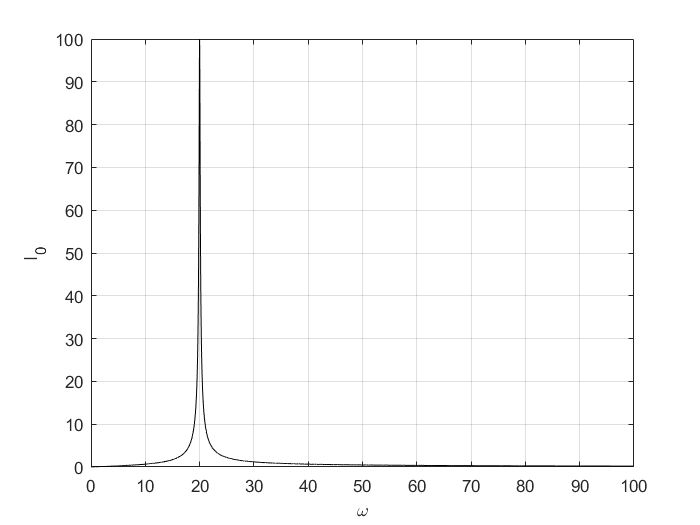
\includegraphics[scale = 0.5]{LRC}\caption{LRC振荡电路谐振曲线($R = 0.01 \Omega, L = 0.05H, C = 0.05F, E_0 = 1V$条件下模拟曲线))}  \label{LRC}
\end{figure}

根据$L (R)C$串联电路的谐振曲线(见图(\ref{LRC}),只有当电动势频率非常接近电路的本征频率,才可以在电路中产生较大的电流,电流对电容充电,$V_C = \frac{1}{C}\int Idt$ 故可以产生较大的电容两端电压,调节可变电容的容值,就可以改变$LRC$ 电路的本征频率,从而使需要的频道的信号在电路中产生最大的电流。

\subsection{检波}
调谐所选择出的信号仍然是高频信号,无法被人耳听到,这里利用包络检波器将高频信号中的低频信息解码出来,图(\ref{circuitOfHomemadeRadio}) 中中间红色矩形框中的电路也就是图(\ref{circuitOfEnvelopeRadio})中所示的电路即为包络检波器的电路图
\begin{figure}
  \centering
  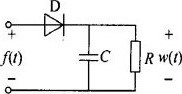
\includegraphics[scale = 1]{circuitOfEnvelopeDetector}\\
  \caption{包络检波器电路图}\label{circuitOfEnvelopeRadio}
\end{figure}
,其主要由一个检波二极管,一个检波电容和一个输出端组成。

其原理如图(\ref{principleOfEnvelopeDetector})
\begin{figure}
  \centering
  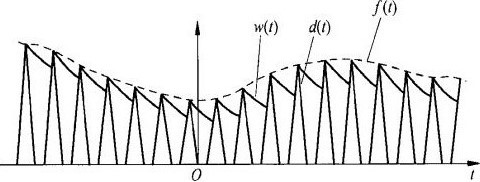
\includegraphics[scale = 0.8]{principleOfEnvelopeDetector(noText)}\\
  \caption{包络检波器原理图}\label{principleOfEnvelopeDetector}
\end{figure}
其中$f(x)$为高频信号的上包络面,$d(t)$为实际的高频信号,$\omega(t)$ 为滤波电容两端的电压。调谐检波二极管将幅值为负的信号部分屏蔽,从而防止对电容器快速正反充电,使正负信号抵消。当二极管导通且感应电动势增大时,对电容器充电,将电容器两端的电压充到接近包络线处,当电路中的电压下降或处于负值而受阻时,电容器两端的电压会有缓慢下降(放电),且这个放电持续的时间相当短,因为高频信号变化得非常得快,等到下一次电路中的电压再次增大时,很快就又将电容器两端的电压充到与包络线附近,从而使得电容器两端的电压一直保持在包络线上,在输出端输出的电压也就是原来的低频信号。图(\ref{principleOfEnvelopeDetector})中为了明显地表示,将电容器两端的电压的变化画得很大,在实际工作中,电容器两端的电压变化得很不明显。

\subsection{利用耳机将处理好的电信号重新转化为声信号}
最常见的耳机是动圈式耳机,其原理为通电导线在磁场中受安培力。耳机的构造与麦克风类似,都是线圈套着永久磁体,线圈中通过的电流的变化使其受到永久磁体的安培力变化,从而产生振动,线圈与振膜相连而带动振膜振动,发出声音。当然耳机的构造不止这一种,还有如同静电耳机,是在两个电容器极板之间加上振膜,振膜以易极化的材料制成,受高电压极化,高电压变化从而产生变化的极化程度,电容器极板之间存在恒定的电场,从而使振膜受到变化的电场力,产生振动,发声。
\subsection{一些对于问题的补充说明}
\subsubsection{关于二极管的放置位置以及电容的设置问题}
由于当二极管导通的时候,两个电容并联,其电容值相加,也就是说两个电容共同充当$LRC$电路中的$C$,也就是说,电路中的二极管无论是接在可变电容器前面还是接在可变电容器后面,都不会对电路的正常工作、耳机两端的电压造成太大影响,这可以通过实验和电路模拟来验证。

但为什么不用一个较大的可变电容来代替我们所制作的电路中的一个小的可变电容加一个大的定值电容?因为根据$LRC$电路共振公式反推,我国无线电广播的频率范围为$535kHz-1605kHz$,不妨设为$1000kHz$,电容器的容值在$2200pF-2230pF$,不妨近似为$2200pF$,解得自制的天线的电感为
\[
L = \frac{1}{4\pi^2\times2200\times{10}^{-12}F\times(1000\times{10}^{3}Hz)^2} \approx 1.15\times{10}^{-5}H
\]
天线电感不变,则只要电容容值能够在$2200pF-2230pF$这么小的范围内调节,就可以覆盖频道范围
\[
\begin{split}
&993845Hz = \frac{1}{2\pi\sqrt{2230\times{10}^{-12}F\times1.15\times{10}^{-5}}}\\
&\leq f \leq\\
&\frac{1}{2\pi\sqrt{2200\times{10}^{-12}F\times1.15\times{10}^{-5}}} = 100599Hz
\end{split}
\]
而如果直接采用几千皮法的大电容,则可能难以进行精细调节,易错过所需要的本振频率。
\subsubsection{采用高阻耳机或用变压器来代替高组耳机的原因}
收音机中使用高组耳机而非普通的电阻耳机是因为,普通的低阻耳机的阻值一般为$16-64\Omega$,而高阻耳机的阻值可达上千欧,最常见的是$2200\Omega$,如前所述,当二极管未导通时,电路左边形成一个无源的$RC$振荡电路,$RC$振荡电路的本征频率为
\[
f = \frac{1}{2\pi RC}
\]
$R$越大,$RC$振荡电路的本征频率就越小,或者说,当二极管未导通时,$RC$振荡电路放电,电容器极板上的电量的变化情况为
\[
Q(t) = Q_0e^{-\frac{t}{CR}}
\]
$R$越大,则$Q(t)$趋向于$0$的速度越慢,即电容器放电时电压下降速度越慢。

若使用低阻耳机,则电容器放电时电压下降速度很快,既很难使电容器两端电压值贴近高频信号包络线,且电容器电压振荡很快,导致音质不佳。

也可以这样看,无论是高电阻还是电感很大的变压器的初级线圈,其阻抗(感抗)很大,可以分到电路中更压的电压,从而减小了电路中的损耗电阻上的电压,从而减小了损耗电阻的功率,余下的功率只能由耳机来消耗。(注意,变压器是一种效率很高的电子元件,经查阅资料得普通变压器的效率普遍在$95\%$以上,故新加的变压器不会消耗很多电能,除了串联电阻消耗的能量,其余大部分能量可以集中到耳机上)
\subsubsection{收音机解调电路的方程}
设天线电感为$L_1$,电阻为$R_1$,通过天线的电磁波所产生的磁通量为$\Phi_B$(以从右向左为正),可变电容为$C_1$,定值电容为$C_1$,可变电容所在支路中的电流为$I_1$(以从上向下为正),定值电容所在支路中的电流为$I_2$ (以从上向下为正)。

若使用高阻耳机,设耳机的电阻为$R$,电容为$C$,电感为$L$,通过耳机的电流为$I_3$(从上到下为正),则当二极管导通时,电路方程为
\[
\begin{split}
&R_1(I_1 + I_2 + I_3) + \frac{1}{C_1}\int I_1dt = - \frac{d\Phi_B}{dt} - L_1\frac{d(I_1 + I_2 + I_3)}{dt}\\
&R_1(I_1 + I_2 + I_3) + \frac{1}{C_2}\int I_2dt = - \frac{d\Phi_B}{dt} - L_1\frac{d(I_1 + I_2 + I_3)}{dt}\\
&R_1(I_1 + I_2 + I_3) + R_3I_3 + \frac{1}{C_3}\int I_3dt = - \frac{d\Phi_B}{dt} - L_1\frac{d(I_1 + I_2 + I_3)}{dt} - L_2\frac{dI_3}{dt}
\end{split}
\]
当二极管未导通时,二极管右边形成一个$LRC$振荡电路,定值电容缓慢漏电,且注意到$I_2 = - I_3$,方程为
\[
C_2\int I_3dt + RI_3 + \frac{C_3}\int I_3dt = - I\frac{dI_3}{dt}
\]
当然,由于在二极管未导通时,各电容器、电感的充放电、磁的情况各有所不同,所以实际解方程时需要注意各个电流的初始值。

若使用变压器来连接普通低阻耳机,不妨设变压器为理想变压器,设初级线圈的电感为$L_2$,次级线圈的电感为$L_3$,由于耦合系数为$1$,故互感$M = \sqrt{L_1L_2}$,通过变压器的初级线圈的电流为$I_3$ (以从上向下为正),耳机的电阻为$R$,电容为$C$,电感为$L$,通过耳机的电流为$I_4$ (以从上向下为正),设电流为所设方向时,变压器的两个线圈产生的磁场同向,当二极管导通时,左边电路的方程组为
\[
\begin{split}
&R_1(I_1 + I_2 + I_3) + \frac{1}{C_1}\int I_1dt = - \frac{d\Phi_B}{dt} - L_1\frac{d(I_1 + I_2 + I_3)}{dt}\\
&R_1(I_1 + I_2 + I_3) + \frac{1}{C_2}\int I_2dt = - \frac{d\Phi_B}{dt} - L_1\frac{d(I_1 + I_2 + I_3)}{dt}\\
&R_1(I_1 + I_2 + I_3) = - \frac{d\Phi_B}{dt} - L_1\frac{d(I_1 + I_2 + I_3)}{dt} - L_3\frac{dI_3}{dt} - M\frac{dI_4}{dt}
\end{split}
\]
当二极管未导通时,二极管右边为一$LC$振荡电路,定值电容缓慢漏电,注意到$I_2 = I_3$,方程为
\[
\frac{1}{C}\int I_3dt = - \frac{dI_3}{dt} - M\frac{dI_4}{dt}
\]
二极管左边亦为一$LC$振荡电路,方程为
\[
R_1I_1 + \frac{1}{C_1}\int I_1dt = - \frac{d\Phi_B}{dt} - L_1\frac{dI_1}{dt}
\]
右边耳机所在电路的方程为
\[
RI_4 +  \frac{1}{C}\int I_4dt = - (L_2 + L)\frac{dI_4}{dt} - M\frac{dI_3}{dt}
\]
\subsubsection{收音机功率计算}
通过查阅资料仅得到上海$FM$调频广播电台的功率及方位(网址:\\\verb|http://www.crystalradio.cn/forum.php?mod=viewthread&tid=149868&archive=3&extra=&page=1)|\\
,但我们所制作的收音机为调幅收音机,我们不妨假设调幅电台的功率、辐射距离与调频相当,用调频电台的数据进行运算,资料中调频收音机的功率一般在$1kW$到$10kW$数量级,一座大城市(上海)城区的半径在几十$km$数量级(但是注意一个电台的广播不一定能覆盖整个城区),我们所制作的收音机的线圈面积约为$0.1m^2$,不妨设通过线圈的电磁波的能量全部转化为电能,且无线广播电台天线并非向空间所有角度发射电磁波,而是向“四周”(不含“向上”和“向下”),故不妨近似波面为一半圆面,由此有收音机的功率
\[
W = \frac{2\times10^4W\times0.1m^2}{2\pi\times(5\times{10}^{3})^2} \approx 1.3\times{10}^{-5}W = 1.27\times{10}^{-2}mW
\]
同时查阅淘宝网商品信息可以得到,一般入耳式耳机最大功率在$mW$的数量级,且其灵敏度在$100dB/mW$的数量级,在平时使用时耳机分贝最高尚处于$10dB$的数量级,即其功率应处于$0.1mW$的数量级,远远小于耳机的最大功率,将耳机用于无源收音机时,听到的信号显然远比正常使用时微弱,由于使用的是高阻耳机,或增设变压器,故耳机两端分到了电路中绝大多数的电压,可以近似视为耳机的功率为$1.27\times{10}^{-2}mW$,与其正常使用的功率相比,较为合理。
\end{document}
